\section{Prelab Code:}
\begin{verbatim}
%% Prelab:
close all
clear all

% Prelab Problem 2:
Fs = 1e6;
t = 0:1/Fs:0.01 - 1/Fs; % 5 seconds
f = 20E3; % 20 Khz

A_c = 5;

f_m = 5E2;
x = sin(2*pi*f_m*t);

f_c = 20E3;
y = A_c*(1+0.5*x).*cos(2*pi*f_c*t);

subplot(3, 2, 1);
plot(t, x);
title('Modulating Signal');
xlabel('Time(in s)');
ylabel('Voltage(in V)');

subplot(3, 2, 2);
plot(t, y);
title('Amplitude Modulated Signal');
xlabel('Time (in s)');
ylabel('Voltage (in V)');

% Frequency spectrum
N = length(y);
Y = fft(y);

spectrum = abs(Y/N);
spectrum_single = spectrum(1:N/2+1);
spectrum_single(1:end-1) = 2*spectrum_single(1:end-1);

F = Fs * (0:(N/2)) / N;
subplot(3, 2, 3);
plot(F, spectrum_single);
xlim([1.9E4, 2.1E4]);
title('Amplitude Modulated Signal Frequency Spectrum');
xlabel("Frequency(in Hz)")
ylabel("Amplitude(in V)")

frequencies = logspace(3, 5, 100); % 100 Hz to 100 KHz
Wn = 1000/(Fs/2); % Normalized cutoff frequency

[b1, a1] = butter(1, Wn); % Butterworth filter of first order
[b3, a3] = butter(3, Wn); % Butterworth filter of third order

% Rectify the signal

% We can use an envelope detector for this, the simplest analogue to a
% diode would be the absolute value of the signal, so that's what will be
% used

% (Ac + abs(Ac)) / 2;
% Or -0.5 for the diode effect
rectified = (A_c + abs(y)) / 2 - 0.5;
filtered = filter(b1, a1, rectified);

% figure;
subplot(3, 2, 4);
plot(t, filtered);
title('First-Order Demodulated Signal');
xlabel('Time(in s)');
ylabel('Voltage(in V)');

filtered3 = filter(b3, a3, rectified);
subplot(3, 2, 5);
plot(t, filtered3);
title('Third-Order Demodulated Signal');
xlabel('Time(in s)');
ylabel('Voltage(in V)');

% Bode plot for the filters
figure;
freqs(b1, a1);
title("First Order Butterworth Filter Bode Plot");

figure;
freqs(b3, a3);
title("Third Order Butterworth Filter Bode Plot");

%% Evaluation: Part 2
close all
clc

w_c = 20E3 * 2 * pi;
w_m = 5E2 * 2 * pi;
c = 5*sin(w_c*t);
y = (1 + 0.70*cos(w_m * t)) .* c;

N = length(y);
Y = fft(y);

spectrum = abs(Y/N);
spectrum_single = spectrum(1:N/2+1);
spectrum_single(1:end-1) = 2*spectrum_single(1:end-1);

F = Fs * (0:(N/2)) / N;
plot(F, 20*log10(spectrum_single / sqrt(2)));
xlim([1.9E4, 2.1E4]);
title('Amplitude Modulated Signal Frequency Spectrum');
xlabel("Frequency(in Hz)")
ylabel("Amplitude(in V)")
\end{verbatim}

\section{Prelab 6}

\subsection{Problem 1}
Knowing that the change of frequency in FM is defined as,
\begin{equation}
    \frac{d\theta}{dt} = \omega_c + k_f m(t) = w_c + k_f 4\cos(8000\pi t)
\end{equation}

And knowing that cosine can, at most, be 1, and at the minimum be -1, we can define the frequency deviation to be(for $f - 4k_f, f + 4k_f$):

\begin{equation}
    \Delta f = 4k_f = 4\cdot 10^4\text{Hz} = 40\text{KHz}
\end{equation}

And knowing that the modulation index is defined as:
\begin{equation}
    m = \frac{\Delta \omega}{\omega_m} = \frac{2\pi 40\text{KHz}}{8000 \pi\text{Hz}} = \frac{2\pi 40000\text{Hz}}{8000\pi\text{Hz}} = 10
\end{equation}

Therefore, the signal is overmodulated.

\newpage
\subsection{Problem 2}
The tables are provided below. The plot is provided as well. There are more peaks whose amplitudes are under -40dB, but they are not shown in the plot, nor in the table. The code used to generate the plot and the table is provided further down in the appendix.

Carlston's rule is used to obtain the bandwidth of the signal.
\begin{equation}
    B_T \simeq 2f_m(\beta + 1)
\end{equation}

Where $\beta$ will be referred to as $m$ in this calculation,
\begin{itemize}
    \item For $m=0.2$, it is found that the bandwidth is 12KHz.
    \item For $m=1$, it is found that the bandwidth is 20KHz.
    \item For $m=2$, it is found that the bandwidth is 30KHz.
\end{itemize}

\begin{figure}[H]
    \centering
    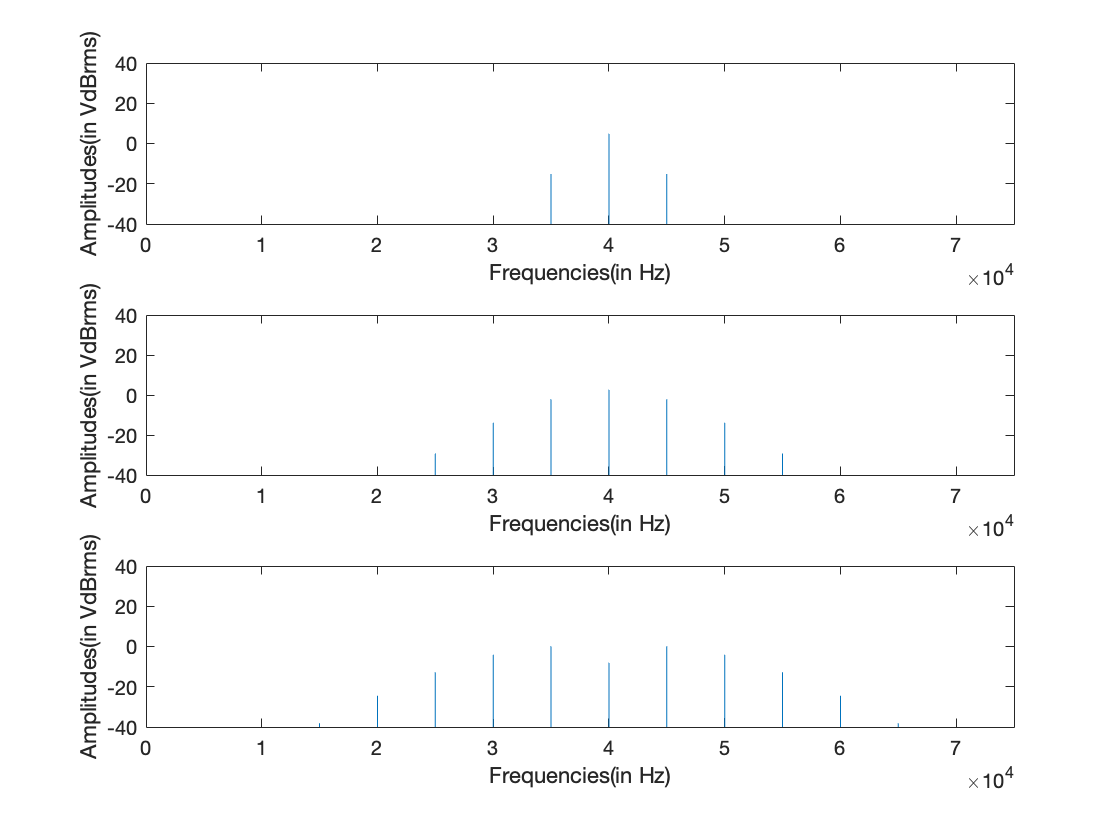
\includegraphics[width=0.75\textwidth]{images/prelab_6_plot.png}
    \label{fig:prelab_06}
    \caption{Frequency spectra for m=0.2, m=1, m=2}
\end{figure}

\begin{table}[H]
    \centering
    \begin{tabular}{|c|l|l|}
        \hline
        \multirow{4}{*}{\textbf{m=0.2}} & \textbf{Frequency(in Hz)} & \textbf{Amplitude(in VdBRms)} \\ \cline{2-3}
                                        & 3501                      & -15                           \\ \cline{2-3}
                                        & 4000                      & 5                             \\ \cline{2-3}
                                        & 4501                      & -15                           \\ \hline
                                        & \textbf{Frequency(in Hz)} & \textbf{Amplitude(in VdBRms)} \\ \hline
        \multirow{4}{*}{\textbf{m=1}}   & 4001                      & 3                             \\ \cline{2-3}
                                        & 4501                      & -2                            \\ \cline{2-3}
                                        & 5001                      & -14                           \\ \cline{2-3}
                                        & 5501                      & -29                           \\ \hline
                                        & \textbf{Frequency(in Hz)} & \textbf{Amplitude(in VdBRms)} \\ \hline
        \multirow{11}{*}{\textbf{m=2}}  & 1501                      & -38                           \\ \cline{2-3}
                                        & 2001                      & -24                           \\ \cline{2-3}
                                        & 2501                      & -13                           \\ \cline{2-3}
                                        & 3001                      & -4                            \\ \cline{2-3}
                                        & 3501                      & 0                             \\ \cline{2-3}
                                        & 4001                      & -8                            \\ \cline{2-3}
                                        & 4501                      & 0                             \\ \cline{2-3}
                                        & 5001                      & -4                            \\ \cline{2-3}
                                        & 5501                      & -13                           \\ \cline{2-3}
                                        & 6001                      & -24                           \\ \cline{2-3}
                                        & 6501                      & -38                           \\ \hline
    \end{tabular}
\end{table}

The decibel values in the table are rounded to the nearest integer.

\subsection{Problem 3}
The circuit turns an FM signal into an AM signal, and then uses a slope detector in order to follow the envelope of the signal. The circuit is re-created using LTSpice to find the bode plot of the circuit. The bode plot and the circuit in LTSpice is provided below. The circuit's behaviour seems to be a bandpass filter.

\begin{figure}[H]
    \centering
    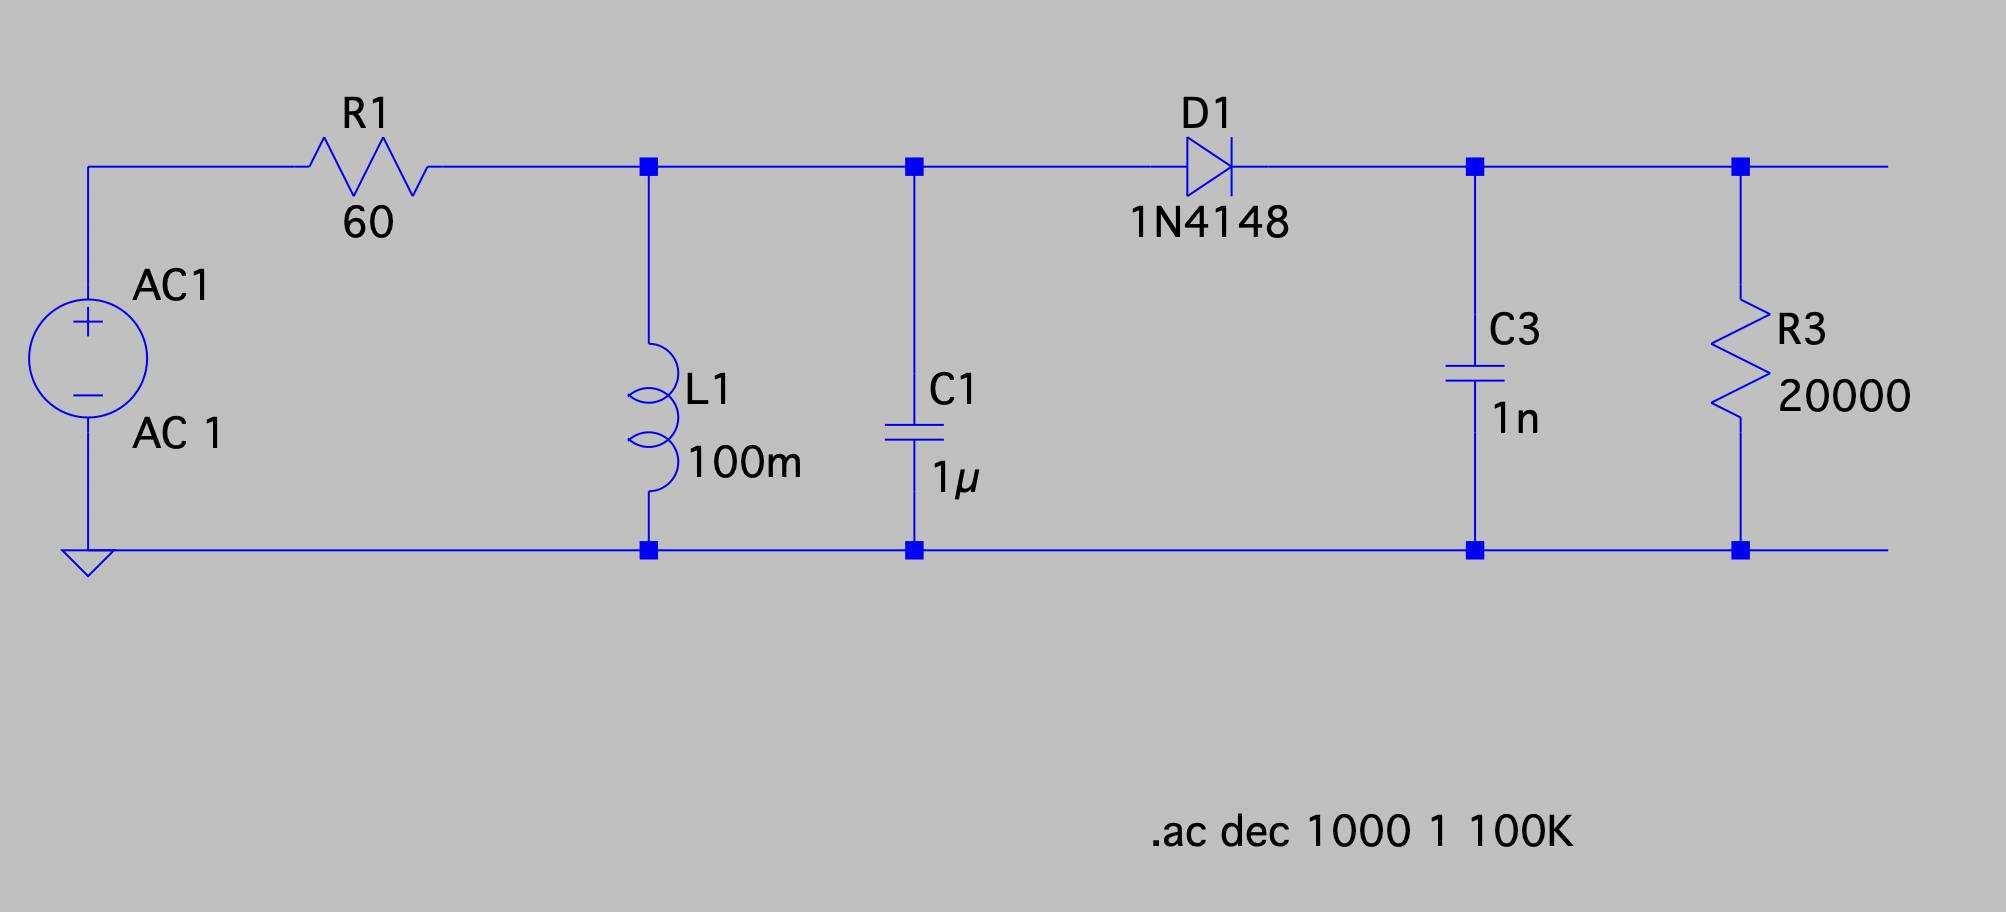
\includegraphics[width=0.75\textwidth]{images/prelab_6_circuit.png}
    \label{fig:prelab_06_circuit}
    \caption{Circuit in LTSpice}
\end{figure}

\begin{figure}[H]
    \centering
    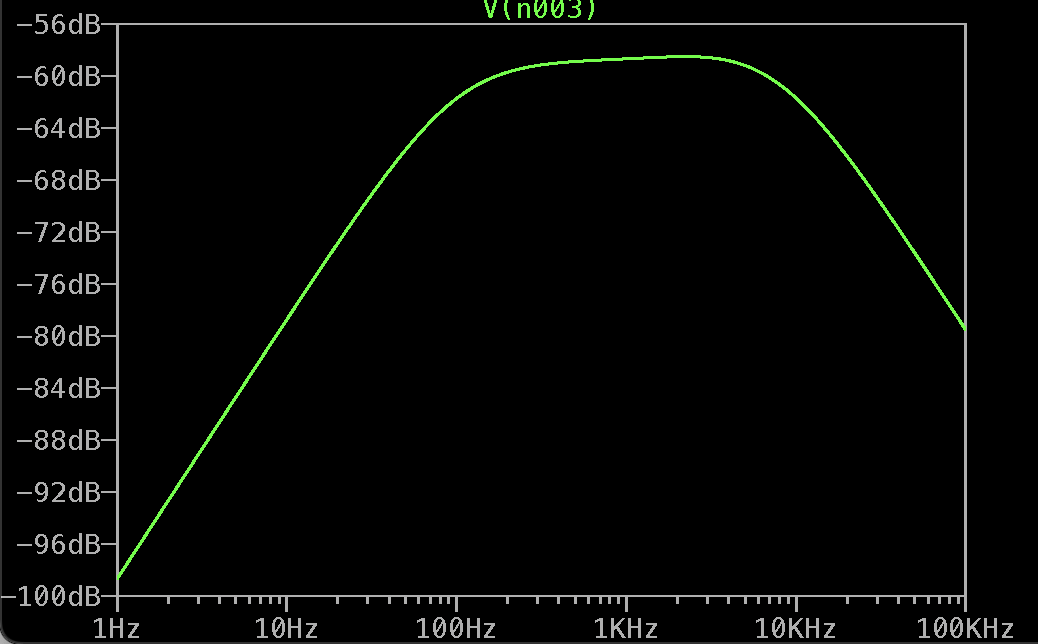
\includegraphics[width=0.75\textwidth]{images/prelab_6_bandpass.png}
    \label{fig:prelab_06_bandpass}
    \caption{Bode plot of the circuit}
\end{figure}

The code for the prelab is provided.
\begin{verbatim}
%% Prelab 6:

Fs = 1E6;
t = 0:1/Fs:0.1-(1/Fs);
w_c = 40E3 *2*pi;
w_m = 5E3*2*pi;

% For m = 0.2
m = 0.2;
y = 2.5.*cos(w_c.*t + m.*sin(w_m.*t));

% subplot(3, 1, 1);
% plot(t, y);

N = length(y);
Y = fft(y);

spectrum = abs(Y/N);
spectrum_single = spectrum(1:N/2+1);
spectrum_single(1:end-1) = 2*spectrum_single(1:end-1);

F = Fs * (0:(N/2)) / N;
subplot(3, 1, 1);

BT = w_m/pi*(0.2+1);
disp("Bandwidth for m=0.2");
disp(BT);

m_02_dB = 20*log10(spectrum_single / sqrt(2));
disp("For m=0.2, peaks are");
display_peaks(m_02_dB);

plot(F, m_02_dB);
xlabel("Frequencies(in Hz)");
ylabel("Amplitudes(in VdBrms)");
xlim([0, 75000]);
ylim([-40, 40]);

% For m = 1
m = 1;
y = 2.5.*cos(w_c.*t + m.*sin(w_m.*t));

N = length(y);
Y = fft(y);

spectrum = abs(Y/N);
spectrum_single = spectrum(1:N/2+1);
spectrum_single(1:end-1) = 2*spectrum_single(1:end-1);

F = Fs * (0:(N/2)) / N;
subplot(3, 1, 2);

m_1_dB = 20*log10(spectrum_single / sqrt(2));

BT = w_m/pi*(1+1);
disp("Bandwidth for m=1");
disp(BT);
disp("For m=1, peaks are");
display_peaks(m_1_dB);

plot(F, m_1_dB);
xlabel("Frequencies(in Hz)");
ylabel("Amplitudes(in VdBrms)");
xlim([0, 75000]);
ylim([-40, 40]);

% For m = 2
m = 2;
y = 2.5.*cos(w_c.*t + m.*sin(w_m.*t));

N = length(y);
Y = fft(y);

% BT ~=2fm(B + 1)
BT = w_m/pi*(2+1);
disp("Bandwidth for m=2");
disp(BT);

spectrum = abs(Y/N);
spectrum_single = spectrum(1:N/2+1);
spectrum_single(1:end-1) = 2*spectrum_single(1:end-1);

F = Fs * (0:(N/2)) / N;
m_2_dB = 20*log10(spectrum_single / sqrt(2));

% Peaks:
disp("For m=2, peaks are:");
display_peaks(m_2_dB);

subplot(3, 1, 3);
plot(F, m_2_dB);
xlabel("Frequencies(in Hz)");
ylabel("Amplitudes(in VdBrms)");
xlim([0, 75000]);
ylim([-40, 40]);

function [] = display_peaks(m_dB)
    frequencies = find(m_dB > -40); % more than -40dB
    decibels = m_dB(frequencies);
    for i = 1:length(frequencies)
        fprintf("Frequency: %d Hz, Decibel: %f dB\n", frequencies(i), round(decibels(i)));
    end
end    
\end{verbatim}